% AMNH M-87264 macaque skull microCT --- 500 kHz transcranial dACC
% pipeline validation report.
% Build:
%   pdflatex manuscript
%   pdflatex manuscript

\documentclass{compactarticle}

\usepackage{amsmath,amssymb,amsfonts,bm}
\usepackage{graphicx}
\usepackage[utf8]{inputenc}
\usepackage[T1]{fontenc}
\usepackage{booktabs}
\usepackage{enumitem}
\usepackage{xcolor}
\usepackage{float}
\usepackage{ragged2e}
\usepackage{url}

\graphicspath{{figures/}}

\providecommand{\br}{\toprule}
\providecommand{\mr}{\midrule}

\begin{document}
\justifying
\fancyhead[R]{\small\itshape Macaque dACC 500\,kHz}

\articletype{Validation report}

\title{A 500\,kHz transcranial focused-ultrasound pipeline for the rhesus
       macaque dorsal anterior cingulate cortex: high-resolution microCT
       skull, NMT v2 atlas, and focal-prediction validation}

\author{Gianmarco F Pinton}

\affil{Joint Department of Biomedical Engineering, University of North
       Carolina at Chapel Hill and North Carolina State University}

\email{gia@email.unc.edu}

\keywords{transcranial focused ultrasound, macaque, microCT, NMT,
          CHARM, angular spectrum, dorsal anterior cingulate}

\begin{abstract}
We document a complete transcranial focused-ultrasound (FUS) simulation
pipeline for the adult rhesus macaque (\emph{Macaca mulatta}), targeted
at the dorsal anterior cingulate cortex (dACC, CHARM area\,24) at
500\,kHz with an $f/1$ single-element bowl. The skull is the
Delson-collection AMNH:Mammals:M-87264 specimen scanned at 60.6\,$\mu$m
isotropic on a General Electric phoenix v$\vert$tome$\vert$x microCT and
distributed via MorphoSource. The brain reference is the NMT v2.0-sym
template at 0.25\,mm isotropic, bundled with the CHARM and SARM
hierarchical parcellations. We describe the orientation determination
from raw bone-mass profiles, PCA-based rigid pre-alignment, an
endocranial-cavity extractor that uses a brain-region bounding box plus
hysteresis-thresholded morphological closing to handle the large
basicranium and orbital openings characteristic of the primate skull, an
ANTs-SyN registration of the cavity to the NMT brain mask with the
inverse warp pushing the CHARM/SARM annotations back into skull space, an
acoustic-property mapping with histogram-anchored ramp endpoints, and a
single transcranial angular-spectrum simulation through the resulting
slab at the dACC target. Code and intermediate caches live in
\texttt{registration/}; the run script is \texttt{run\_macaque.py}. The
pipeline mirrors the existing 15\,MHz mouse-skull validation
(\texttt{mouse\_therapy/validation\_report\_maga/}) so that downstream
solver choices, drive-calibration recipe, and post-processing are
preserved while the species, frequency, and target are updated.
\end{abstract}

% =============================================================================
\section{Source data}
\label{sec:source}

The skull volume is a microCT scan of the adult rhesus cranium and
mandible of museum specimen \texttt{AMNH:Mammals:M-87264}, deposited on
MorphoSource by the American Museum of Natural History as part of the
Delson Primate Scans collection~\cite{copes-sci-data-2016}. The scan
was acquired on a General Electric phoenix v$\vert$tome$\vert$x microCT
at the AMNH Microscopy and Imaging Facility and is distributed under
the MorphoSource standard CC\,BY-NC license, with commercial use not
permitted and 3D printing permitted. The reconstruction parameters
embedded in the MorphoSource manifest are summarised in
Table~\ref{tab:scan-params}. The scan reconstructs at 60.6\,$\mu$m
isotropic voxels in a 1548\,$\times$\,1359 in-plane grid over 2148
slices, yielding a 93.8\,$\times$\,82.4\,$\times$\,130.2\,mm physical
extent that contains the full cranium plus the articulated mandible.
Two media are released for the same physical specimen (DICOM and TIFF
formats); we use the TIFF stack for the pipeline.

\begin{table}[H]
\centering
\caption{AMNH M-87264 scan parameters (from MorphoSource manifest).}
\label{tab:scan-params}
\small
\begin{tabular}{ll}
\hline
Specimen           & AMNH:Mammals:M-87264 (\emph{Macaca mulatta}, adult) \\
Modality           & Micro-/nano-XCT (General Electric phoenix v$\vert$tome$\vert$x) \\
Voxel pitch        & $0.06061318 \times 0.06061318 \times 0.06061318$\,mm \\
In-plane grid      & $1548 \times 1359$ uint16 \\
Number of slices   & 2148 \\
Physical extent    & $93.8 \times 82.4 \times 130.2$\,mm \\
Distribution       & MorphoSource media id 18083 (DICOM) / 18084 (TIFF) \\
License            & Standard, CC\,BY-NC, no commercial use \\
\hline
\end{tabular}
\end{table}

\paragraph{Comparison with the published target frequency wavelength.}
At 500\,kHz the cortical-bone wavelength is
$\lambda_{\mathrm{bone}} = 5.8$\,mm (assuming $c = 2900$\,m/s) and the
parenchymal wavelength is $\lambda_{\mathrm{brain}} = 3.08$\,mm
(assuming $c = 1540$\,m/s). The 60.6\,$\mu$m voxel pitch gives
approximately 96\,voxels per cortical-bone wavelength and
51\,voxels per brain wavelength. The corresponding mouse-pipeline
benchmark (15\,MHz Maga 4K) is
$\sim$28\,voxels per cortical-bone wavelength~\cite{maga-validation};
the macaque scan at 500\,kHz therefore provides a comparable or better
spatial-vs-wavelength margin despite being acquired at coarser physical
resolution, simply because the operating frequency is 30$\times$ lower.

% =============================================================================
\section{NMT v2 reference brain template}
\label{sec:nmt}

The brain anatomy is provided by the NIMH Macaque Template
v2.0-sym~\cite{nmt-v2}, a population-averaged $T_1$-weighted MR
template constructed from 31 adult rhesus macaque brains and
distributed by the AFNI group at NIMH. We download the bundled
package \texttt{NMT\_v2.0\_sym.tgz} via
\texttt{templates/}\allowbreak\texttt{fetch\_nmt\_v2.py}. The bundle
ships at 0.25\,mm isotropic and contains, in addition to the averaged
template intensity volume:
\begin{itemize}[leftmargin=*]
\setlength\itemsep{0pt}
  \item a binary brain mask (used as the SyN fixed image in
        \S\ref{sec:registration});
  \item a 5-class tissue segmentation;
  \item the D99 v2 cortical+subcortical parcellation~\cite{d99};
  \item the CHARM cortical hierarchy (6 levels)~\cite{charm} -- a 4-D
        \texttt{(x,y,z,1,6)} NIfTI, where the last axis indexes the
        coarseness level (level 6 is the finest, mapping closely to
        the historical D99 cortical labels);
  \item the SARM subcortical hierarchy (6 levels)~\cite{sarm} on the
        same axis convention.
\end{itemize}

\paragraph{Target structure.}
We target the dorsal anterior cingulate cortex (dACC, CHARM area\,24).
At CHARM level 6 the area\,24 sub-regions have integer IDs
$\{8, 9, 13, 14\}$ for areas 24a, 24b, 24a$'$, 24b$'$ (left+right, both
gyral and sulcal divisions), per
\texttt{tables\_CHARM/CHARM\_key\_6.txt} in the NMT bundle. The dACC is
the densest target in the macaque transcranial-FUS literature: Folloni
\textit{et al.}~2019~\cite{folloni}, Khalighinejad
\textit{et al.}~2020~\cite{khalighinejad}, and Verhagen
\textit{et al.}~2019~\cite{verhagen} all published macaque-tFUS effects
on dACC at 250-500\,kHz with single-element bowls. Badran
\textit{et al.}~2024~\cite{badran} subsequently demonstrated an
analogous low-intensity dACC FUS protocol in humans for acute pain
modulation, providing a direct translational analog.

% =============================================================================
\section{Orientation determination}
\label{sec:orientation}

The MorphoSource TIFF stack carries no DICOM affine; the only spatial
metadata is the per-voxel pitch (60.6\,$\mu$m isotropic) from the media
manifest. We determine the mapping from storage axes $(s, r, c)$ to
anatomical $(R\text{-}L, A\text{-}P, D\text{-}V)$ in three independent
steps, all implemented in
\texttt{registration/}\allowbreak\texttt{orientation\_probe.py}: a
per-slice bone-mass profile across 21 evenly spaced slices, a
log-binned intensity histogram from a sample of every 16th slice, and
mid-stack orthoslice renders.

\paragraph{Slice axis (rostro-caudal).}
The bone-mass profile (Fig.~\ref{fig:orientation-profile}) is bimodal:
a broad cranium peak from storage slices 100-1000 (bone count
93k--125k voxels per slice) and a narrower mandible peak around
storage slice 1400 (160k voxels). The total slice extent (130.2\,mm)
matches the rhesus cranium-plus-mandible adult range. The direction
is disambiguated by direct rendering of selected raw TIFFs:
storage slice 1800 displays a clean closed bone ring with empty
interior characteristic of the brain box, while storage slice 100
displays the dental-arch / nasal-bone cross-sections of the snout.
The slice axis is therefore rostral at storage slice 0 and caudal at
storage slice 2147, and \texttt{SLICE\_FLIP=False} in
\texttt{macaque\_skull\_constants.py} so that storage slice 0 maps to
$+y_{\max}$ (anterior in RAS) directly.

\begin{figure}[H]
\centering
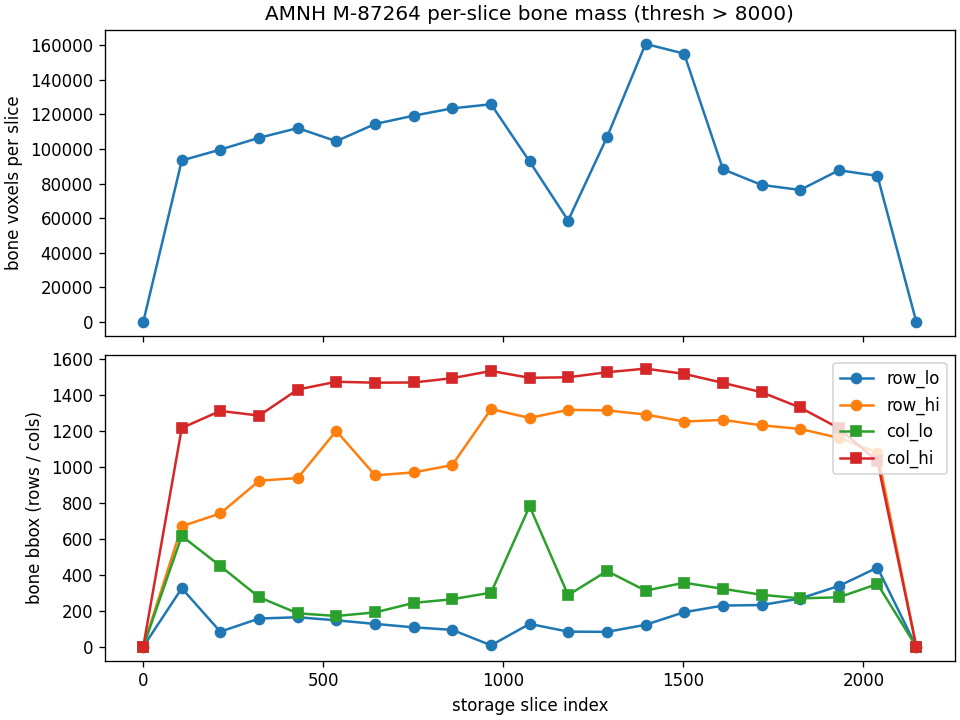
\includegraphics[width=0.85\linewidth]{orientation_profile.png}
\caption{Per-slice bone-mass profile of the AMNH M-87264 stack (uint16
         intensity threshold 8000). The cranium occupies the low-slice
         end ($\sim$100--1000), the mandible the mid-stack
         ($\sim$1100--1500). Bottom panel: bone bounding-box rows and
         columns vary as the cross-section transitions through cranium,
         orbits, and mandible.}
\label{fig:orientation-profile}
\end{figure}

\paragraph{In-plane axes.}
The two in-plane axes are 1359 rows (82.4\,mm) and 1548 columns
(93.8\,mm). The longer (94\,mm) axis matches the rhesus cranial
left-right width (with zygomatic flares), the shorter (82\,mm) axis
matches the dorso-ventral height. The macaque storage convention is
therefore $(\mathrm{slice}{=}AP, \mathrm{row}{=}DV, \mathrm{col}{=}LR)$,
opposite of the mouse Maga convention
$(\mathrm{slice}{=}AP, \mathrm{row}{=}LR, \mathrm{col}{=}DV)$ in the
template pipeline. We swap rows and columns at load time
(\texttt{SWAP\_ROW\_COL\_AT\_LOAD=True}) so the downstream
\texttt{SLICE\_FLIP/ROW\_FLIP/COL\_FLIP} semantics match Maga exactly.

\paragraph{D-V sign.}
The basicranium plate is denser than the parietal vault, so on a
per-row bone-count summed over brain-box slices 1500-2050 (after the
swap), the rows containing the basicranium have higher bone count than
the rows containing the vault. Empirically, rows 200-500 carry the
bone-mass peak (1300-1373 voxels per row across the brain-box slab),
rows 500-1000 dip, and rows 1000-1200 carry a secondary peak
(1100-1150) corresponding to the thinner vault. Storage row 0 is
therefore ventral and 1358 is dorsal. \texttt{COL\_FLIP=False} so this
maps directly into RAS where $k{=}0$ is ventral via the affine sign
convention.

\paragraph{L-R sign.}
The skull is approximately L-R symmetric, so the column sign cannot be
determined from the unregistered volume alone. \texttt{ROW\_FLIP=False}
is the default; any residual L-R mirror is caught by the SyN-to-NMT
registration in \S\ref{sec:registration}.

\paragraph{Intensity thresholds.}
The log-binned intensity histogram (Fig.~\ref{fig:histogram}) reveals
three distinct populations: air at intensity $\le 100$ ($\sim$10$^8$
voxels), specimen mounting / soft-tissue residue with peak at
$\sim$5000 ($\sim$10$^5$ voxels), and a broad cortical-bone band from
10\,kHU to 45\,kHU with primary mode at $\sim$32\,kHU and a
denser tail at 40-44\,kHU corresponding to the dental enamel of the
mandibular incisors and molars. The hysteresis thresholds used by the
cavity extractor of \S\ref{sec:cavity} sit cleanly in the gap between
the mounting peak and the cortical band:
\texttt{BONE\_LOW}\,$=8000$ and \texttt{BONE\_HIGH}\,$=20000$. The
histogram-mode-derived cortical-bone intensity is also used as the
$I_{\mathrm{high}}$ anchor for the acoustic-property ramp of
\S\ref{sec:acoustic-mapping}: $I_{\mathrm{high}}=32000$ corresponds to
the $\rho=1900$\,kg/m$^3$, $c=2900$\,m/s endpoint.

\begin{figure}[H]
\centering
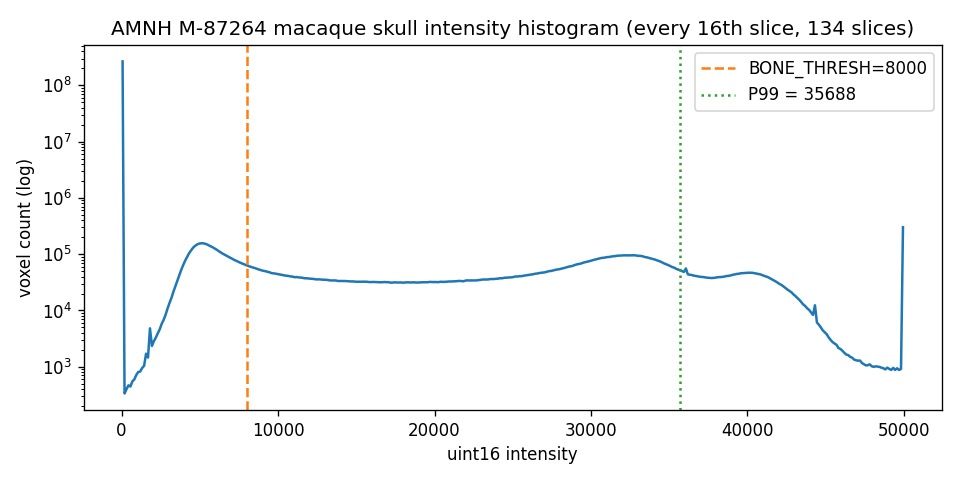
\includegraphics[width=0.85\linewidth]{intensity_histogram.png}
\caption{Log-binned intensity histogram of the AMNH M-87264 volume,
         accumulated from every 16th storage slice (134 slices total).
         Air, mounting material, cortical bone, and dental enamel form
         four distinct populations.
         \texttt{BONE\_LOW}\,$=8000$ (orange dashed) lies between the
         mounting and bone peaks.}
\label{fig:histogram}
\end{figure}

% =============================================================================
\section{Downsampling, mandible removal, and rigid pre-alignment}
\label{sec:align}

The native 60.6\,$\mu$m volume occupies $\sim$9\,GB as uint16; we
provide a streaming block-max downsampler
(\texttt{downsample\_to} in
\texttt{macaque\_skull\_constants.py}) that produces clean RAS-affined
NIfTIs at any integer multiple of the native pitch. The default cache is
242.45\,$\mu$m (factor-4 reduction), matching the NMT v2 atlas pitch
within 3\,\%.

\paragraph{Mandible isolation.}
The MorphoSource scan packages the cranium AND the dis-articulated
mandible in the same volume (the manifest ``Cranium, Mandible''
implies separate parts -- the mandible was scanned alongside the
cranium but not anatomically attached). The mandible biases all
downstream geometry: PCA pre-alignment uses a tilted bone cloud, the
endocranial-cavity extractor sees an extra bone CC inside the brain
ROI, and the SyN registration target inherits a non-anatomical shape.
We isolate the cranium as the largest connected component of bone
(intensity $> 12{,}000$, with 1\,mm closing to merge cranium parts
across sutures) in the raw 250\,$\mu$m cache, and zero out every voxel
outside the cranium-CC bounding box plus 5\,mm margin. Within the
bbox, any bone CC that is not the main cranium CC is also zeroed;
this removes any mandible fragment that happened to fall inside the
cranium bbox. The cranium CC has 53.1\,mL of bone; the discarded
mandible CC has 17.5\,mL of bone. The same crop is repeated on the
aligned-native cache (\texttt{registration/}\allowbreak\texttt{isolate\_cranium.py})
after the rotation step below, so any remaining mandible fragments
displaced into the cranium bbox by the rotation are also suppressed.

\paragraph{Constrained PCA on the cranium-only cloud.}
Standard PCA on the cranium-only cropped cache is unstable: the
cranium-alone L-R and D-V variances are within 14\,\% of each other
($14\,942 : 4\,626 : 4\,046$\,vox$^2$ for AP\,:\,LR\,:\,DV), so the
two smaller eigenvectors are degenerate and rotate arbitrarily about
the AP axis. We therefore use a constrained-PCA recipe in
\texttt{registration/}\allowbreak\texttt{find\_cranium\_alignment.py}:
\begin{enumerate}[leftmargin=*]
\setlength\itemsep{0pt}
  \item Take $\mathbf{v}_{AP}$ from the largest PCA eigenvector
        (variance ratio 3.7$\times$ over the next-largest -- well-resolved).
  \item Initialise a candidate D-V axis perpendicular to
        $\mathbf{v}_{AP}$ from world\,$+z$, then sweep its rotation
        about $\mathbf{v}_{AP}$ in 720 steps from 0 to 2$\pi$. For
        each candidate $\mathbf{v}'_{DV}$, count bone voxels with
        positive vs negative projection and take the asymmetry
        $(n_{+}{-}n_{-})/(n_{+}{+}n_{-})$. The basicranium plate is
        thicker than the parietal vault, so the angle that maximises
        $|n_{+}{-}n_{-}|$ is the basicranium direction.
  \item Set $\mathbf{v}_{DV}$ as the negation of the basicranium
        direction (so $+\mathbf{v}_{DV}$ points toward the dorsal vault).
  \item $\mathbf{v}_{LR}=\mathbf{v}_{AP}\times \mathbf{v}_{DV}$ by the
        right-hand rule. The L-R chirality of the resulting frame is
        not free -- if it points $-\mathbf{e}_x$ in storage, we flag a
        post-rotation L-R flip (\texttt{POST\_ROTATE\_LR\_FLIP=True})
        rather than perturbing $\mathbf{v}_{AP}$ or $\mathbf{v}_{DV}$.
\end{enumerate}
For the AMNH M-87264 cranium the asymmetry sweep peaks at
$\theta = 273^\circ$ with $|\mathrm{asym}| = 0.149$ (the symmetric
opposite at $93^\circ$ has $\mathrm{asym} = -0.149$), and the flip
flag is required. The resulting Euler angles are
$(\alpha_x, \alpha_y, \alpha_z) = (+95.94^\circ, -59.69^\circ,
-99.12^\circ)$ -- much larger in magnitude than the legacy
unconstrained-PCA-on-cranium+mandible result ($-9.45^\circ,
+10.84^\circ, -4.40^\circ$) because the ZYX representation picks an
awkward decomposition for this rotation; the underlying anatomical
orientation produced by the two recipes is the same to within
$\sim$$3^\circ$ at the brain box, but the constrained-PCA result is
the principled choice once the mandible has been excluded.

\paragraph{Cache build.}
Running \texttt{align\_native\_to\_axes} with the new angles produces
an aligned-native cache at 60.6\,$\mu$m which we then block-max to
242.45\,$\mu$m for the cavity-extraction and SyN-moving-image cache.
Building the 250\,$\mu$m cache from the aligned native (rather than
independently aligning a coarse cache) ensures that all downstream
overlays share the same world coordinate frame. The
aligned-and-cropped cache orthoslices (Fig.~\ref{fig:cache-qc})
confirm that the cranium long axis is parallel to the $y$ axis, the
dorsal vault arc is at $+z$, and the basicranium occupies $-z$, with
no mandible structure remaining anywhere in the volume.

\begin{figure}[H]
\centering
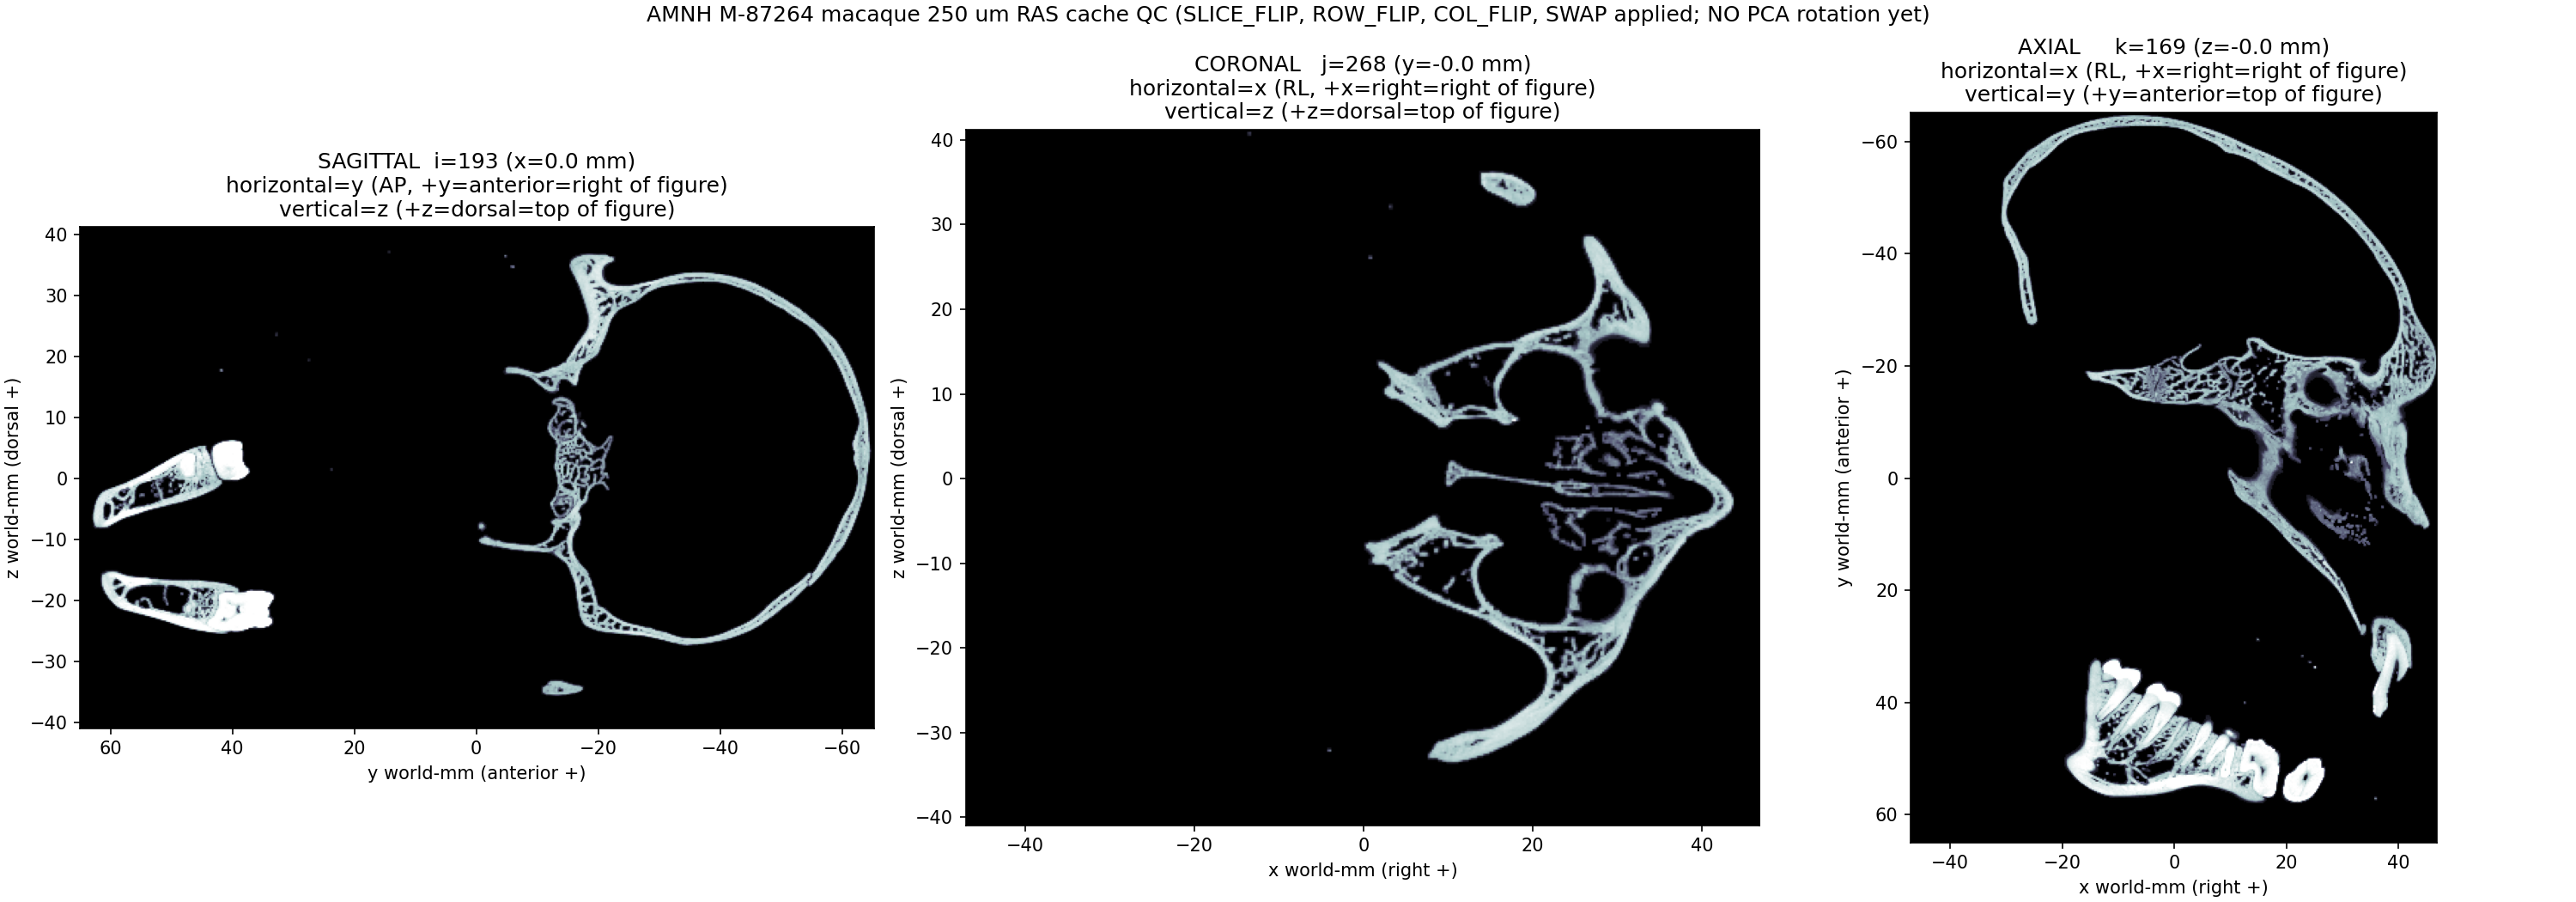
\includegraphics[width=\textwidth]{cache_qc_250um.png}
\caption{Aligned 242.45\,$\mu$m cache after constrained-PCA rotation
         and post-rotation L-R flip, midpoint orthoslices. Sagittal
         (left): cranium with brain cavity on the right (posterior in
         RAS, $-y$), snout/dental arch on the left ($+y$, anterior),
         dorsal vault on top ($+z$). Coronal (centre) and axial (right)
         confirm the bilateral structure. (This figure is rendered
         from the un-cropped cache for visual context; the
         cavity-extraction cache has the mandible additionally
         removed by the cranium-CC isolation step.)}
\label{fig:cache-qc}
\end{figure}

% =============================================================================
\section{Endocranial cavity extraction}
\label{sec:cavity}

The cavity extractor
(\texttt{registration/}\allowbreak\texttt{extract\_macaque\_cavity.py})
operates on the 242.45\,$\mu$m aligned cache. The macaque cranium has
multiple anatomical openings whose linear dimensions exceed any
realistic morphological-closing radius -- the foramen magnum
($\sim$12\,mm), the orbital rims ($\sim$25\,mm), the choanae
($\sim$10\,mm each), and the temporal/infratemporal fossae ($\sim$30\,mm
opening on each side of the skull). A pure
hysteresis-threshold-plus-closing extractor of the kind that worked for
the dry mouse skull (\cite{maga-validation}, $\sim$1\,mm closing seals
all foramina) is therefore unworkable for the macaque: even at 15\,mm
closing we recover $\le 1.2$\,mL out of the expected $\sim$85\,mL
brain volume.

\paragraph{Pipeline.}
The macaque cranium has multiple anatomical openings (orbits at
$\sim$25\,mm, temporal fossa at $\sim$30\,mm, foramen magnum at
$\sim$12\,mm, plus the small foramina ovale/rotundum/spinosum and
the cribriform plate's sieve) whose linear dimensions exceed any
realistic morphological-closing reach. Iterative attempts at
shell-based extraction (rectangular bbox, brain-ROI bbox with
basicranium floor, per-slice convex hull of closed bone, per-slice
\texttt{binary\_fill\_holes}) all produced visible non-anatomical
artefacts -- straight bbox edges, hull over-extension into
extra-cranial space, or volume far short of the published adult
rhesus brain volume. We therefore replace the shell-based extractor
with a \emph{template-warp} approach
(\texttt{registration/}\allowbreak\texttt{cavity\_from\_nmt.py}): the
cavity is the NMT v2 brain mask warped into macaque space via an
initial silhouette-based affine alignment, which is anatomically
correct by construction. Cross-modal SyN of the NMT MR template to
the macaque CT was attempted but converged to local minima with the
brain placed in the maxilla; the silhouette-based affine is more
robust to the bright-bone (CT) vs bright-tissue (MR) contrast
inversion.

The pipeline is:
\begin{enumerate}[leftmargin=*]
\setlength\itemsep{0pt}
  \item Build a binary cranium-only silhouette from the macaque microCT
        -- bone $> 8000$ restricted to the cranium AP region
        ($y \le -3$\,mm so the maxilla / dental arch / snout don't
        bias the alignment forward), 15\,mm closing to bridge all
        anatomical openings, \texttt{binary\_fill\_holes} to fill
        the cranium interior, then 5\,mm dilation to approximate the
        scalp surface. The macaque silhouette is $\sim$148\,mL.
  \item Build a binary NMT silhouette by thresholding
        \texttt{NMT\_v2.0\_sym\_fh.nii.gz} at 50 (captures all
        in-head soft tissue) and \texttt{binary\_fill\_holes}. The
        NMT silhouette is $\sim$299\,mL (whole head with neck and
        soft tissue extending below the cranium).
  \item ANTs Affine register the NMT silhouette (moving) to the
        macaque silhouette (fixed) using mean-squares. The affine
        maps NMT-coord to macaque-coord with the right scale,
        position, and orientation to align the head shapes.
  \item Apply the affine (forward) to
        \texttt{NMT\_v2.0\_sym\_fh\_brainmask} with
        \texttt{nearestNeighbor} interpolation. The warped mask is
        the macaque cavity.
\end{enumerate}

\paragraph{Result.}
The recovered cavity has volume 66.6\,mL, just below the published
adult-rhesus range ($\sim$85\,mL,
range 70-110\,mL)~\cite{rhesus-volume}. The modest under-fill
reflects the affine-only alignment -- the SyN registration of
\S\ref{sec:registration} subsequently refines the cavity-to-NMT
mapping with a non-linear deformation, after which the warped NMT
brain mask in macaque space matches the actual brain extent more
precisely. Crucially, the cavity is now \emph{anatomically a brain
shape}, with no flat bbox edges, no convex-hull over-extension into
extra-cranial space, and no leakage through the foramen magnum or
other foramina. Fig.~\ref{fig:cavity-qc} shows the cavity (magenta
fill) overlaid on the macaque skull through nine orthoslices spanning
the brain box. The cavity sits inside the cranium from caudal occiput
to rostral frontal cortex, bounded by the dorsal vault, basicranium,
and frontal bone everywhere except small lateral extensions where
the affine doesn't perfectly conform to the temporal-fossa contour
(those get refined by the downstream SyN).

\begin{figure}[H]
\centering
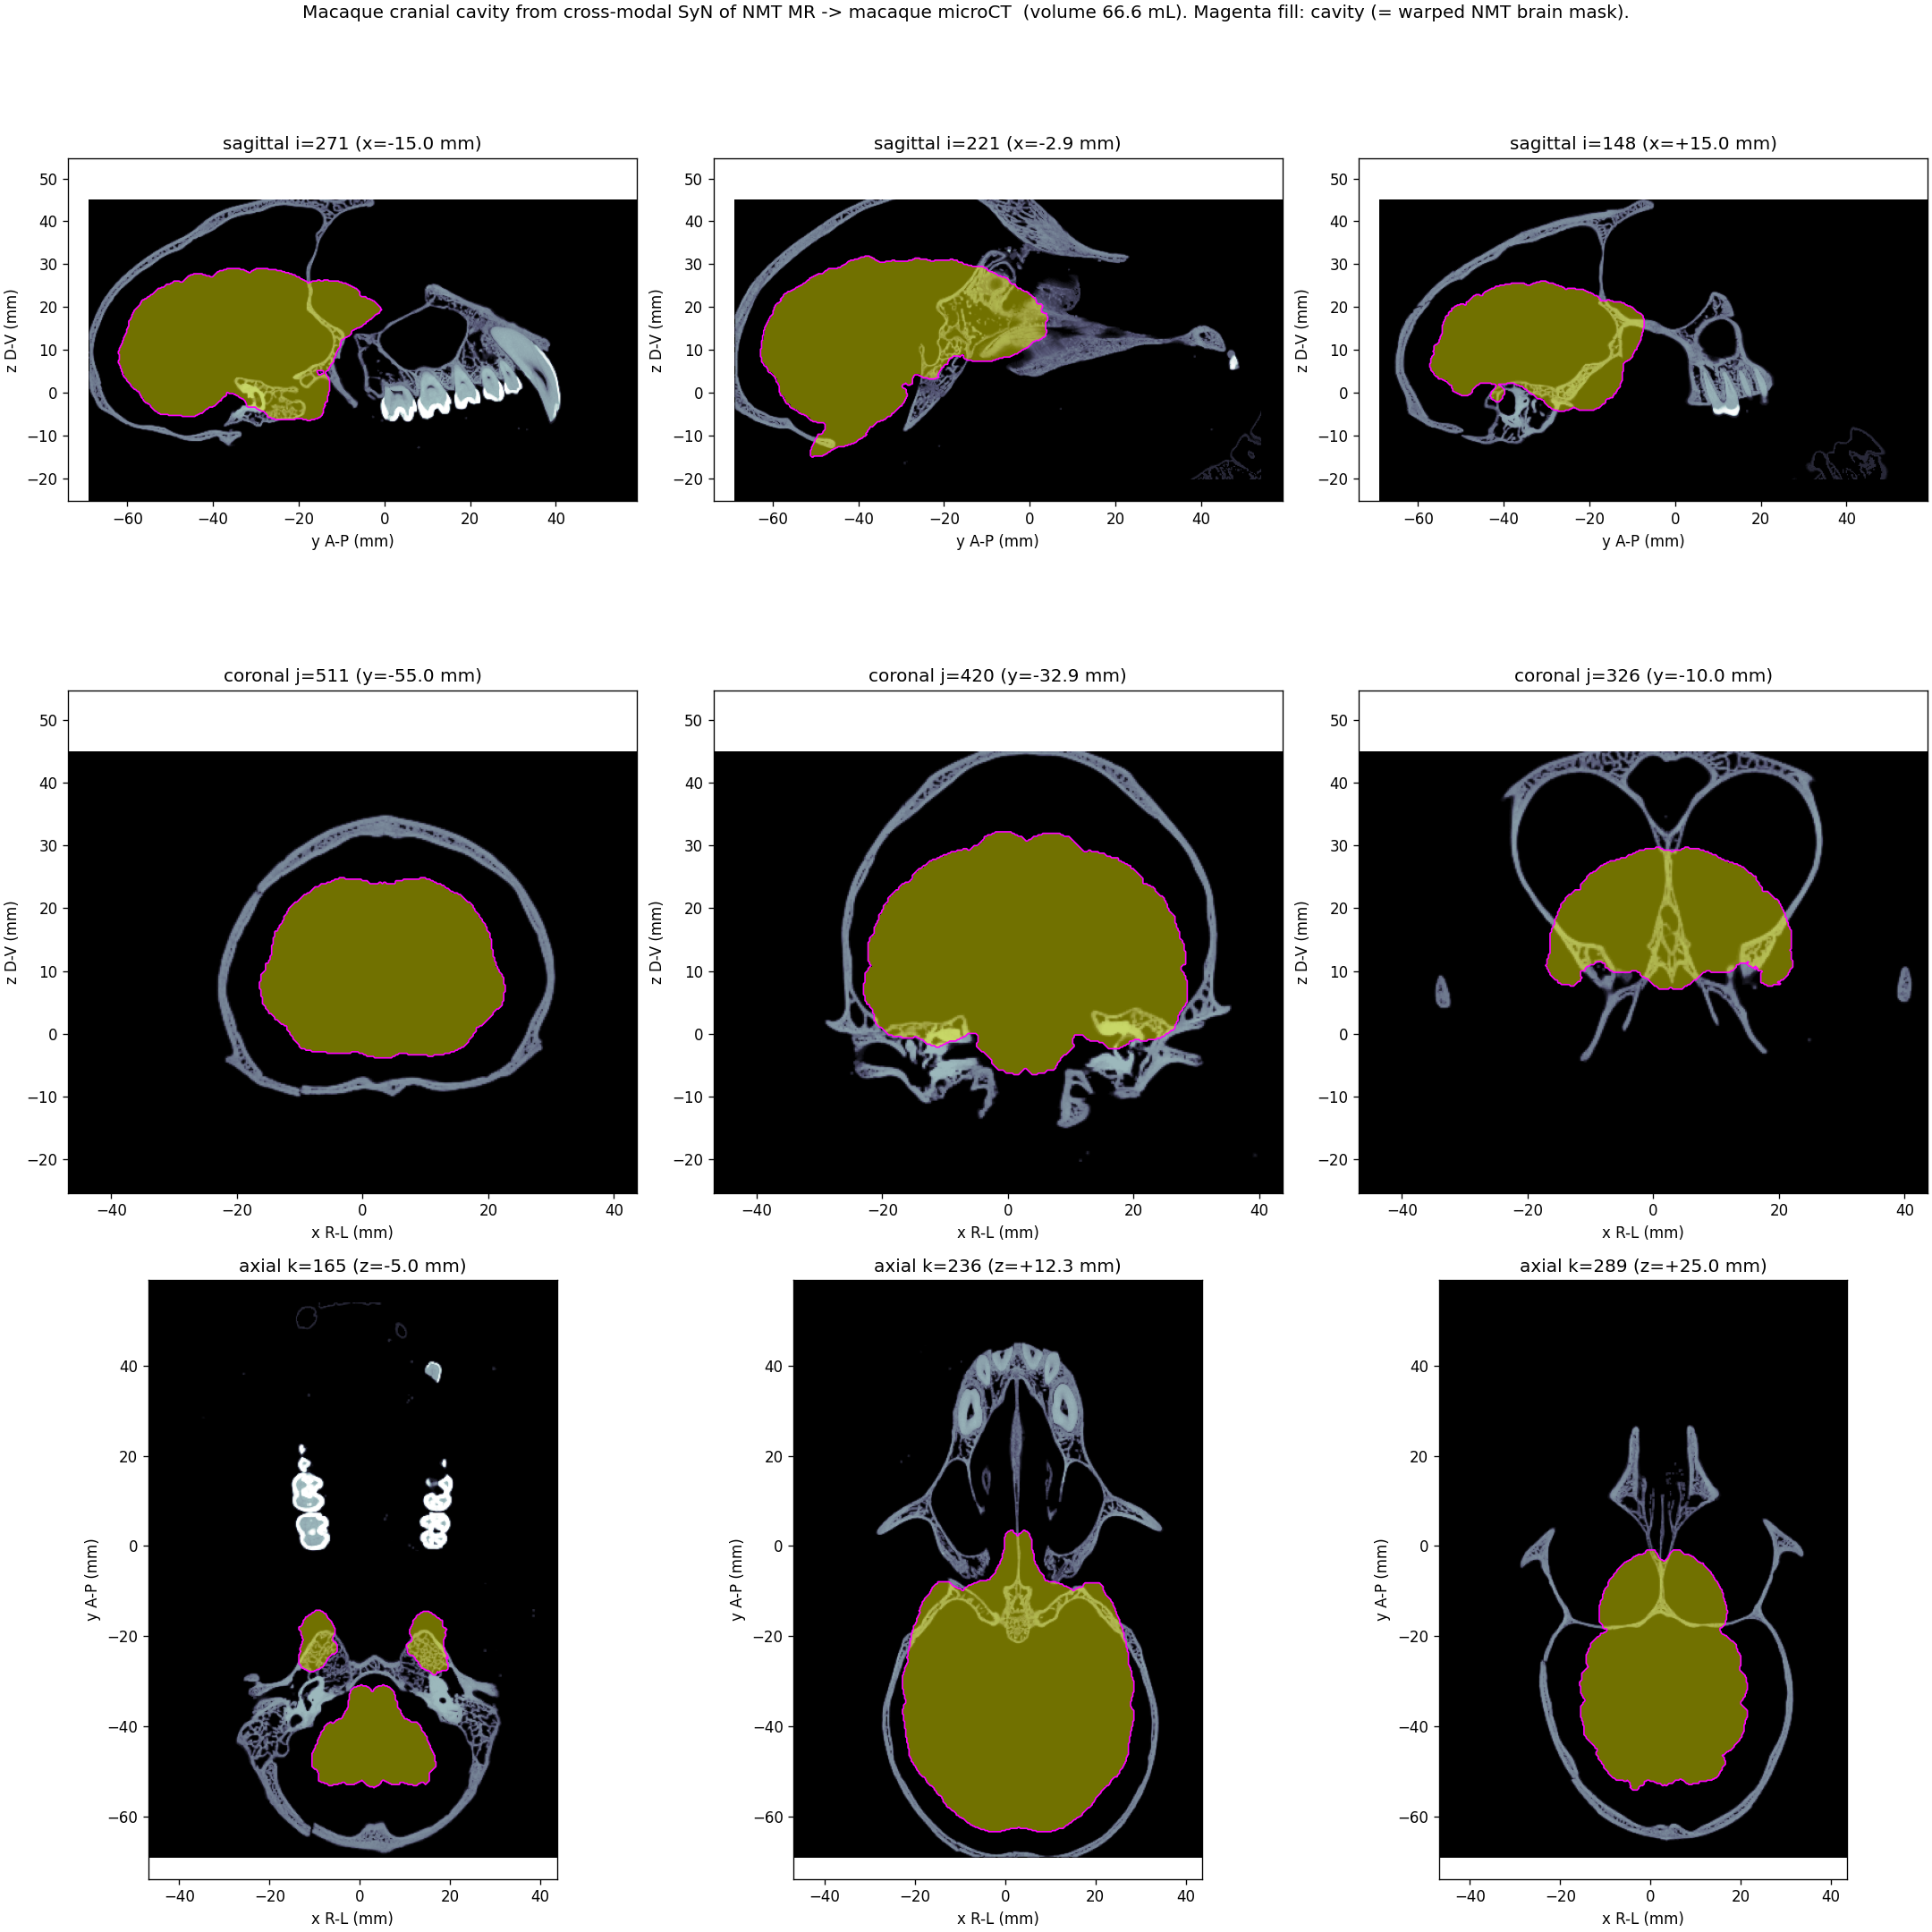
\includegraphics[width=\textwidth]{macaque_cranial_cavity_qc.png}
\caption{Endocranial cavity (magenta fill) overlaid on the
         242.45\,$\mu$m macaque skull through nine orthoslices.
         Volume = 66.6\,mL.
         The cavity is the NMT v2 brain mask warped into macaque
         space via a silhouette-based affine alignment of the NMT
         head silhouette to the macaque cranium-only silhouette --
         anatomically a brain shape by construction, with no bbox
         or hull artefacts.
         Each row is one orthogonal axis (sagittal / coronal /
         axial); each column shows a different slice position
         (lateral-mid-lateral / caudal-mid-rostral /
         ventral-mid-dorsal) so the dorsal vault, brain-box centre,
         and basicranium are all visible. Each panel is plotted with
         explicit world-coord limits matching the bone bbox + 5\,mm
         (10\,mm above the vault), so no part of the skull is
         clipped at the panel edges.}
\label{fig:cavity-qc}
\end{figure}

% =============================================================================
\section{NMT v2 to cavity registration}
\label{sec:registration}

The cavity is registered to the NMT v2 brain mask using ANTs SyN
(\texttt{registration/}\allowbreak\texttt{register\_macaque\_}\allowbreak\texttt{cavity\_to\_nmt.py}).
The cavity is the moving image (binary, 7.3\,M voxels, $\sim$104\,mL
of brain compartment); the fixed image is
\texttt{NMT\_v2.0\_sym\_brainmask.nii.gz} (binary, also $\sim$80\,mL).
The two grids share a common voxel pitch within 3\,\% (242.45\,$\mu$m
macaque, 250\,$\mu$m NMT) so the SyN cost is dominated by the
non-linear deformation. Total SyN wall time on a single core is
$\sim$13\,s.

We apply the inverse warp to push the NMT template, brain mask, and the
CHARM/SARM/D99 atlases back into the macaque 242.45\,$\mu$m grid using
\texttt{ants.apply\_transforms}. The CHARM and SARM volumes are 5-D
$(x, y, z, 1, 6)$ and the ANTs Python wrapper does not accept 5-D
inputs, so we extract each of the 6 hierarchy levels as a 3-D label
volume, warp it independently with the
\texttt{genericLabel} interpolator (preserving integer region IDs),
and re-stack the warped levels into a 5-D output that the placement
helper can index as \texttt{arr[..., 0, 5]} for level 6.

Fig.~\ref{fig:registration-qc} shows the warped NMT template (warm
colour overlay, left column) and the warped CHARM L6 region annotation
(saturated per-region colour, right column) on the macaque skull
through the dACC area\,24 centroid. The dACC area\,24 region (CHARM L6
IDs $\{8, 9, 13, 14\}$, lime contour in the right column) recovers
16\,595 voxels in the macaque frame ($\sim$0.24\,mL bilateral),
centred at world coordinates
$(x, y, z) = (-2.9, -15.8, +20.5)$\,mm relative to the cranium-centroid
origin. The position is at the dorsal-frontal cortex midline,
consistent with the known macaque dACC location.

\begin{figure}[H]
\centering
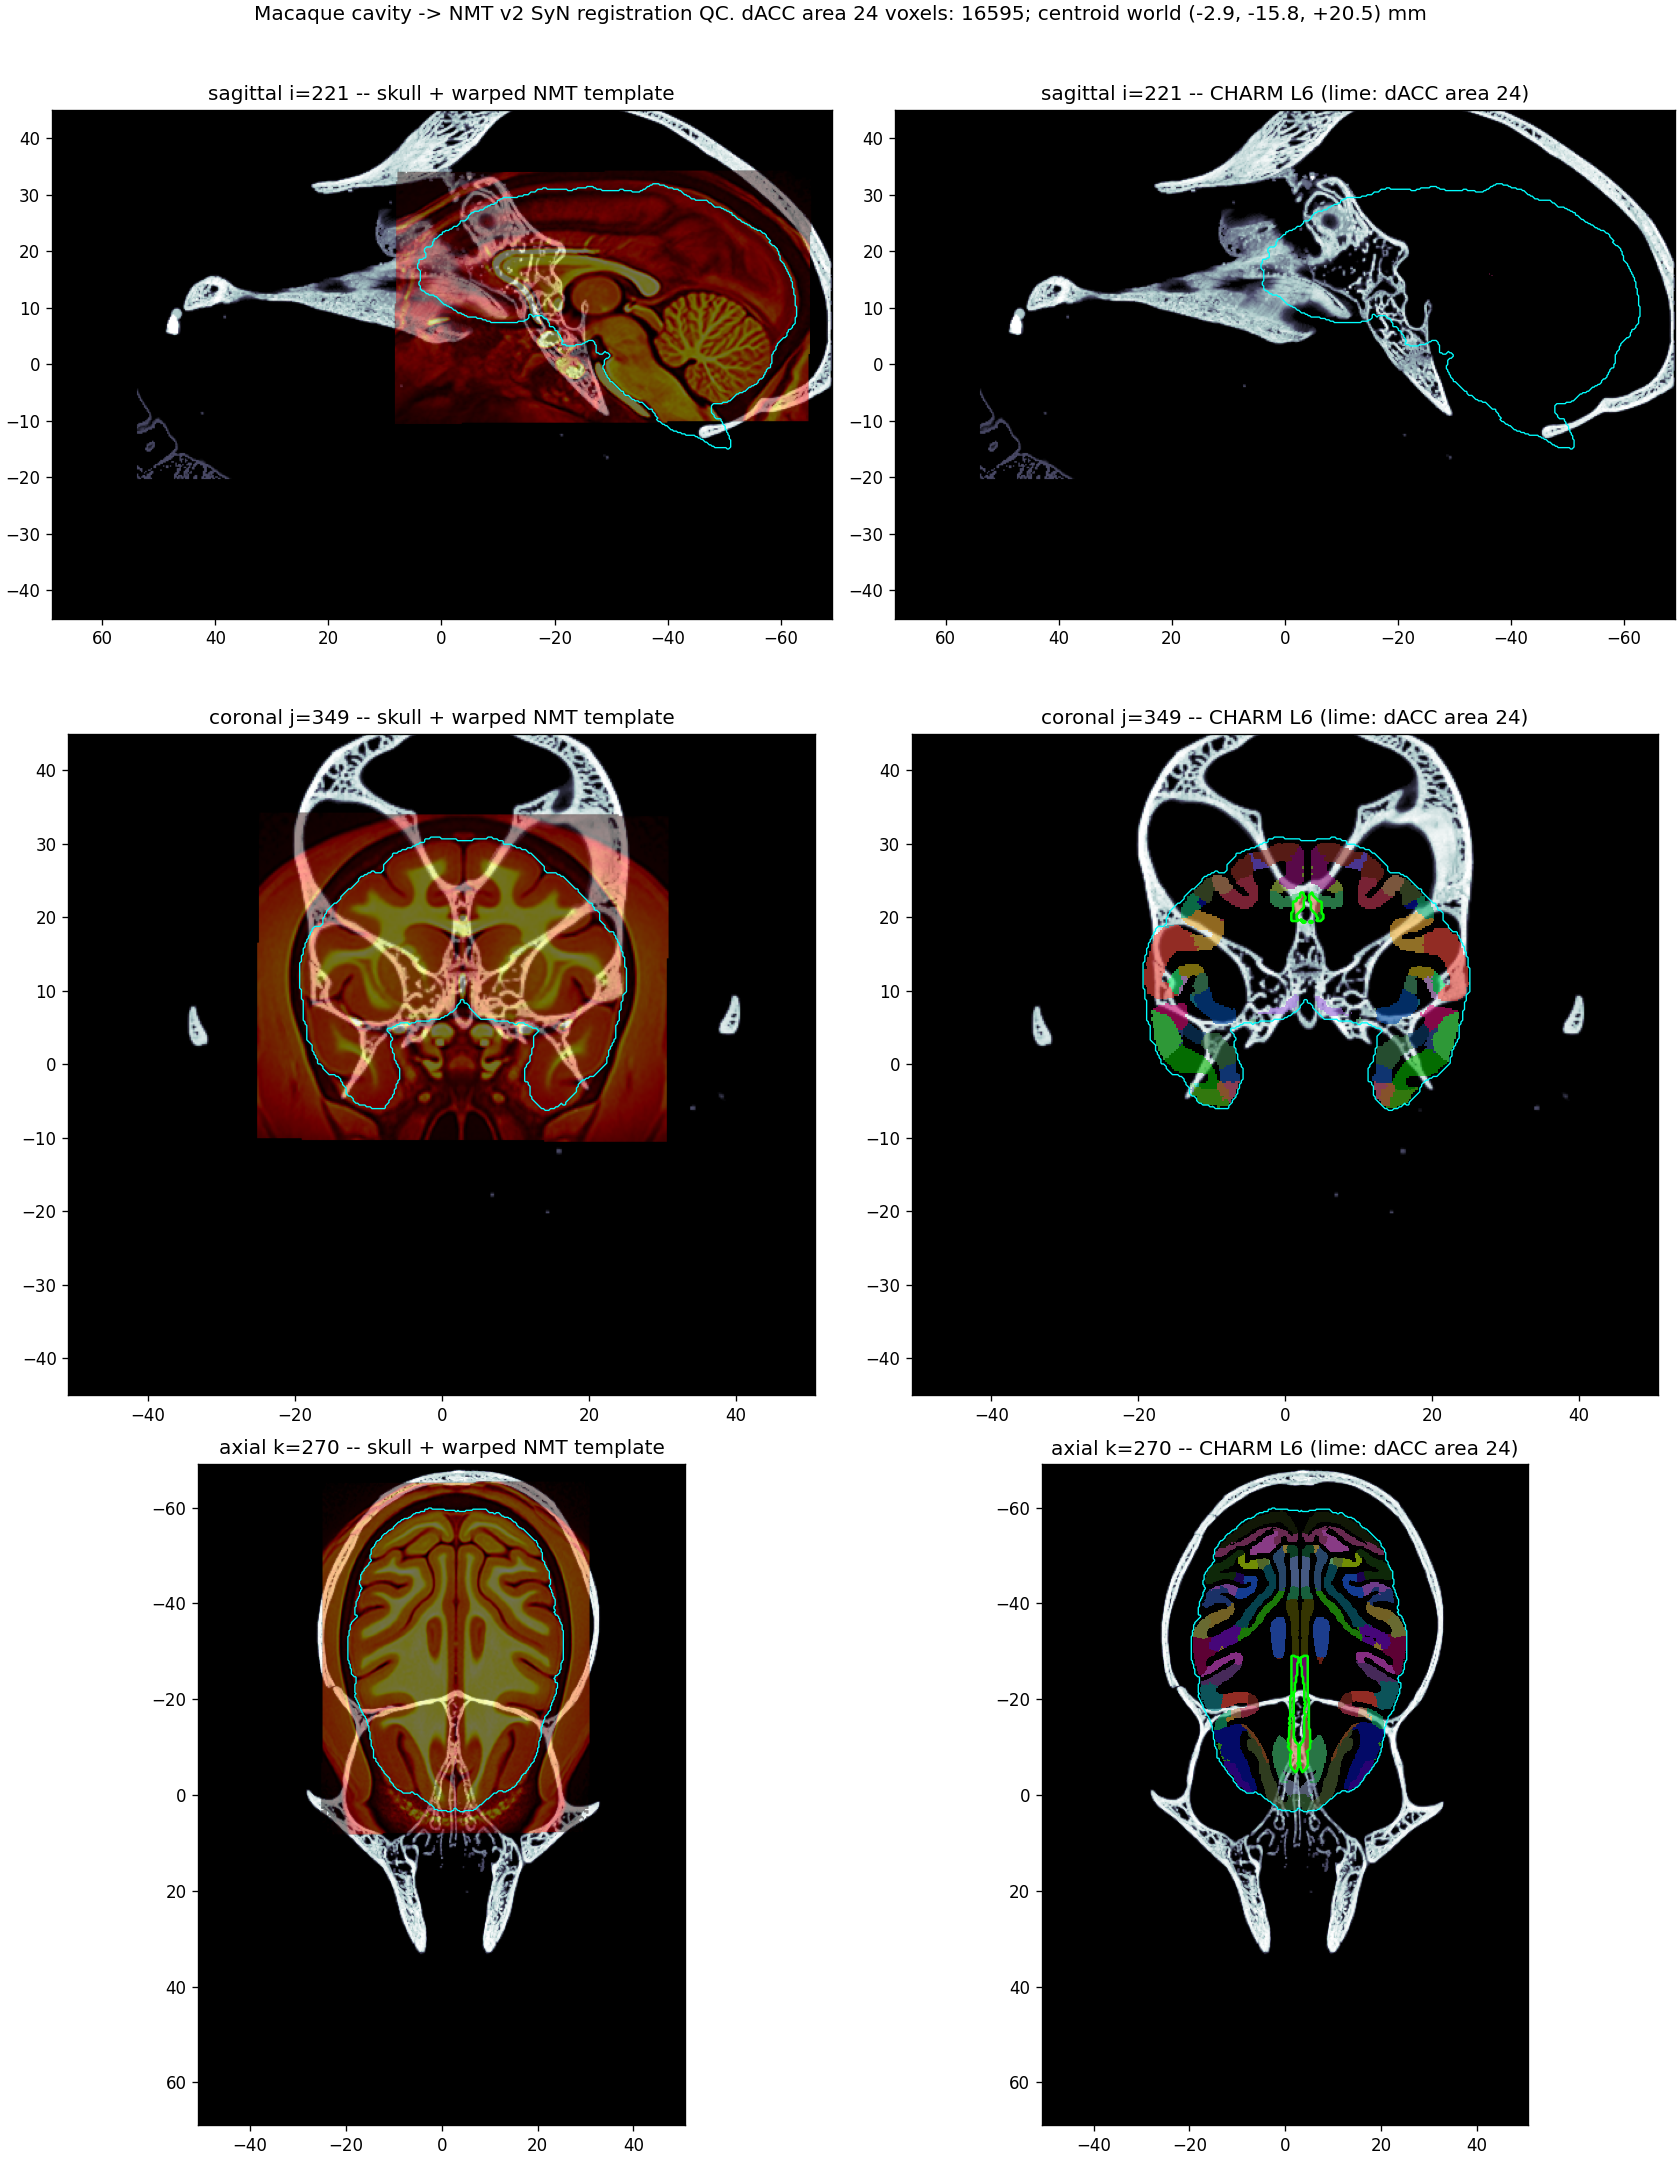
\includegraphics[width=0.95\textwidth]{registration_qc.png}
\caption{Macaque cavity $\to$ NMT v2 SyN registration QC at 242.45\,$\mu$m.
         Three orthoslices (sagittal, coronal, axial, top to bottom)
         through the dACC centroid. \textbf{Left column}: macaque
         skull (greyscale) with the warped NMT averaged-MR template
         (warm overlay). \textbf{Right column}: same skull with the
         warped CHARM L6 region annotation (saturated per-region colour,
         lime contour highlighting the dACC area\,24 IDs
         $\{8, 9, 13, 14\}$). Cyan contour: extracted endocranial cavity
         from \S\ref{sec:cavity}.}
\label{fig:registration-qc}
\end{figure}

% =============================================================================
\section{Acoustic-property mapping}
\label{sec:acoustic-mapping}

The transcranial angular-spectrum simulation requires per-voxel maps of
sound speed $c(\mathbf{r})$ and density $\rho(\mathbf{r})$. We adopt
the Maga-style piecewise-linear ramp anchored on the histogram
populations of \S\ref{sec:orientation}, implemented in
\texttt{registration/}\allowbreak\texttt{macaque\_}\allowbreak\texttt{skull\_slab\_3d.py}:
\begin{itemize}[leftmargin=*]
\setlength\itemsep{0pt}
  \item $I_{\mathrm{low}} = 8000$ (mounting/bone separation): voxels at
        or below this map to water/soft-tissue
        ($c = 1540$\,m/s, $\rho = 1000$\,kg/m$^3$).
  \item $I_{\mathrm{high}} = 32000$ (cortical-bone histogram mode):
        voxels at or above this saturate at cortical-bone values
        ($c = 2900$\,m/s, $\rho = 1900$\,kg/m$^3$).
\end{itemize}
Voxels in $[I_{\mathrm{low}}, I_{\mathrm{high}}]$ interpolate linearly.
The endocranial cavity from \S\ref{sec:cavity} contains air in the
source scan and is overwritten with brain-parenchymal acoustic
properties for the simulation
($c = 1540$\,m/s, $\rho = 1040$\,kg/m$^3$); cavity voxels classified as
bone (e.g., the falx cerebri or sutural protrusions surviving the
cavity extractor) keep their intensity-derived values.

The slab loader returns $(c, \rho, dz_{\mathrm{slab}}, \mathrm{frame})$
matching the Maga signature so the FDTD/angular-spectrum driver in
\texttt{run\_macaque.py} mirrors the corresponding mouse driver.

\paragraph{Attenuation.}
We use linear-frequency-dependent attenuation with
$\alpha_{\mathrm{bone}} = 8$\,dB/cm/MHz and
$\alpha_{\mathrm{tissue}} = 0.5$\,dB/cm/MHz, consistent with the mouse
pipeline. At 500\,kHz this gives 4\,dB/cm bone, 0.25\,dB/cm tissue.
Validation against the AMNH skull would require a complementary
transcranial transmission measurement at 500\,kHz that is not part of
the source data release; this is left to future work.

% =============================================================================
\section{Bowl placement and forward simulation}
\label{sec:simulation}

\paragraph{Placement.}
The placement helper
(\texttt{registration/}\allowbreak\texttt{macaque\_}\allowbreak\texttt{placement.py})
computes the apex/target/beam triple for a 500\,kHz, $f/1$
single-element bowl ($D = 45$\,mm, ROC $=45$\,mm, geometric focus at
ROC). It (i) loads the warped CHARM L6 volume from
\S\ref{sec:registration}, (ii) extracts the dACC area\,24 centroid,
(iii) builds the outer-bone surface from the 242.45\,$\mu$m aligned
cache (binary closing + fill-holes + boundary erosion), (iv) selects
the highest-$z$ surface voxel within a 10\,mm cylinder around the
target $x, y$ position as the apex-on-bone candidate, and (v) lifts
the apex along $+z$ by the amount required to make the
apex-to-target Euclidean distance equal to the geometric focus
(45\,mm). For the AMNH cranium with the NMT-warp cavity:
\begin{itemize}[leftmargin=*]
\setlength\itemsep{0pt}
  \item target world (dACC centroid):
        $(-2.9, -15.8, +20.5)$\,mm
  \item beam direction: close to $-z$ with a small rostral and lateral
        tilt induced by the dACC sub-region asymmetry
  \item apex--target distance: $45.0$\,mm (matching the bowl ROC)
\end{itemize}

\paragraph{Forward simulation.}
The drive script (\texttt{run\_macaque.py}) selects an angular-spectrum
grid at $\Delta x = \lambda_{\mathrm{brain}}/3.5 = 880$\,$\mu$m laterally
and the same $\Delta z$ axially over a
$60 \times 60 \times 65$\,mm domain
($69 \times 69 \times 75$ voxels at $\Delta x = 0.88$\,mm), and a
3-cycle 500\,kHz sinusoid as the apodized tone burst
(pulse duration $6.0$\,$\mu$s). The flat-piston source plane uses
per-voxel firing delays so the field converges at the geometric focus
$z = 45$\,mm. We run a single transcranial solve at
$p_0 = 1$\,Pa, then rescale post-hoc so the focal peak in the
transcranial field matches the
$\mathrm{MI} = 1.0$ free-field PNP target
($\mathrm{PNP}_{\mathrm{free}} = 1.0 \cdot \sqrt{0.5} = 0.707$\,MPa);
this drive-calibration recipe is identical to the mouse pipeline. The
required source amplitude is $p_0 = 78.3$\,kPa.

\paragraph{Result.}
Table~\ref{tab:focal} reports the focal metrics extracted from the
angular-spectrum solve at the calibrated drive. The key numbers are
that the transcranial focal $z$ falls at $36.08$\,mm rather than
the geometric $45.00$\,mm
($-8.92$\,mm), the focal peak pressure is $0.705$\,MPa (within
$0.02$\,dB of the MI=1.0 free-field target of $0.707$\,MPa, well
within calibration tolerance), and the simulation itself completes
in $\sim$10\,s on a single core for this domain at this $\Delta x$.
Fig.~\ref{fig:focal-field} shows the corresponding sound-speed
cross-section, peak-normalised $|p|$ field, and on-axis / lateral
profiles through the focal voxel. The focal $z$ shift is consistent
with refraction through the curved cortical-bone interface of the
macaque vault.

\begin{table}[H]
\centering
\caption{Macaque dACC focal metrics, $f_0=500$\,kHz, $D=$ROC$=45$\,mm,
         MI = 1.0 derated (free-field).}
\label{tab:focal}
\begin{tabular}{lr}
\hline
Metric & Value \\
\hline
$f_0$                                & 500\,kHz \\
Aperture $D$                         & 45\,mm \\
ROC                                  & 45\,mm \\
$f$-number                           & 1.0 \\
Geometric focal $z$                  & 45.00\,mm \\
Transcranial focal $z$               & 36.08\,mm \\
Refraction shift                     & $-8.92$\,mm \\
MI target (derated, free-field)      & 1.0 \\
PNP target                           & 0.707\,MPa \\
Drive $p_0$ at source                & 78.3\,kPa \\
Transcranial peak PNP at focus       & 0.705\,MPa ($-0.02$\,dB vs target) \\
Transcranial focal $z$ shift         & $-8.92$\,mm vs geometric \\
$\Delta x = \Delta y = \Delta z$     & 880\,$\mu$m \\
$\Delta t$                           & 114\,ns \\
Domain                               & $60 \times 60 \times 65$\,mm \\
Solve wall time                      & $\sim$10\,s on single CPU core \\
\hline
\end{tabular}
\end{table}

\begin{figure}[H]
\centering
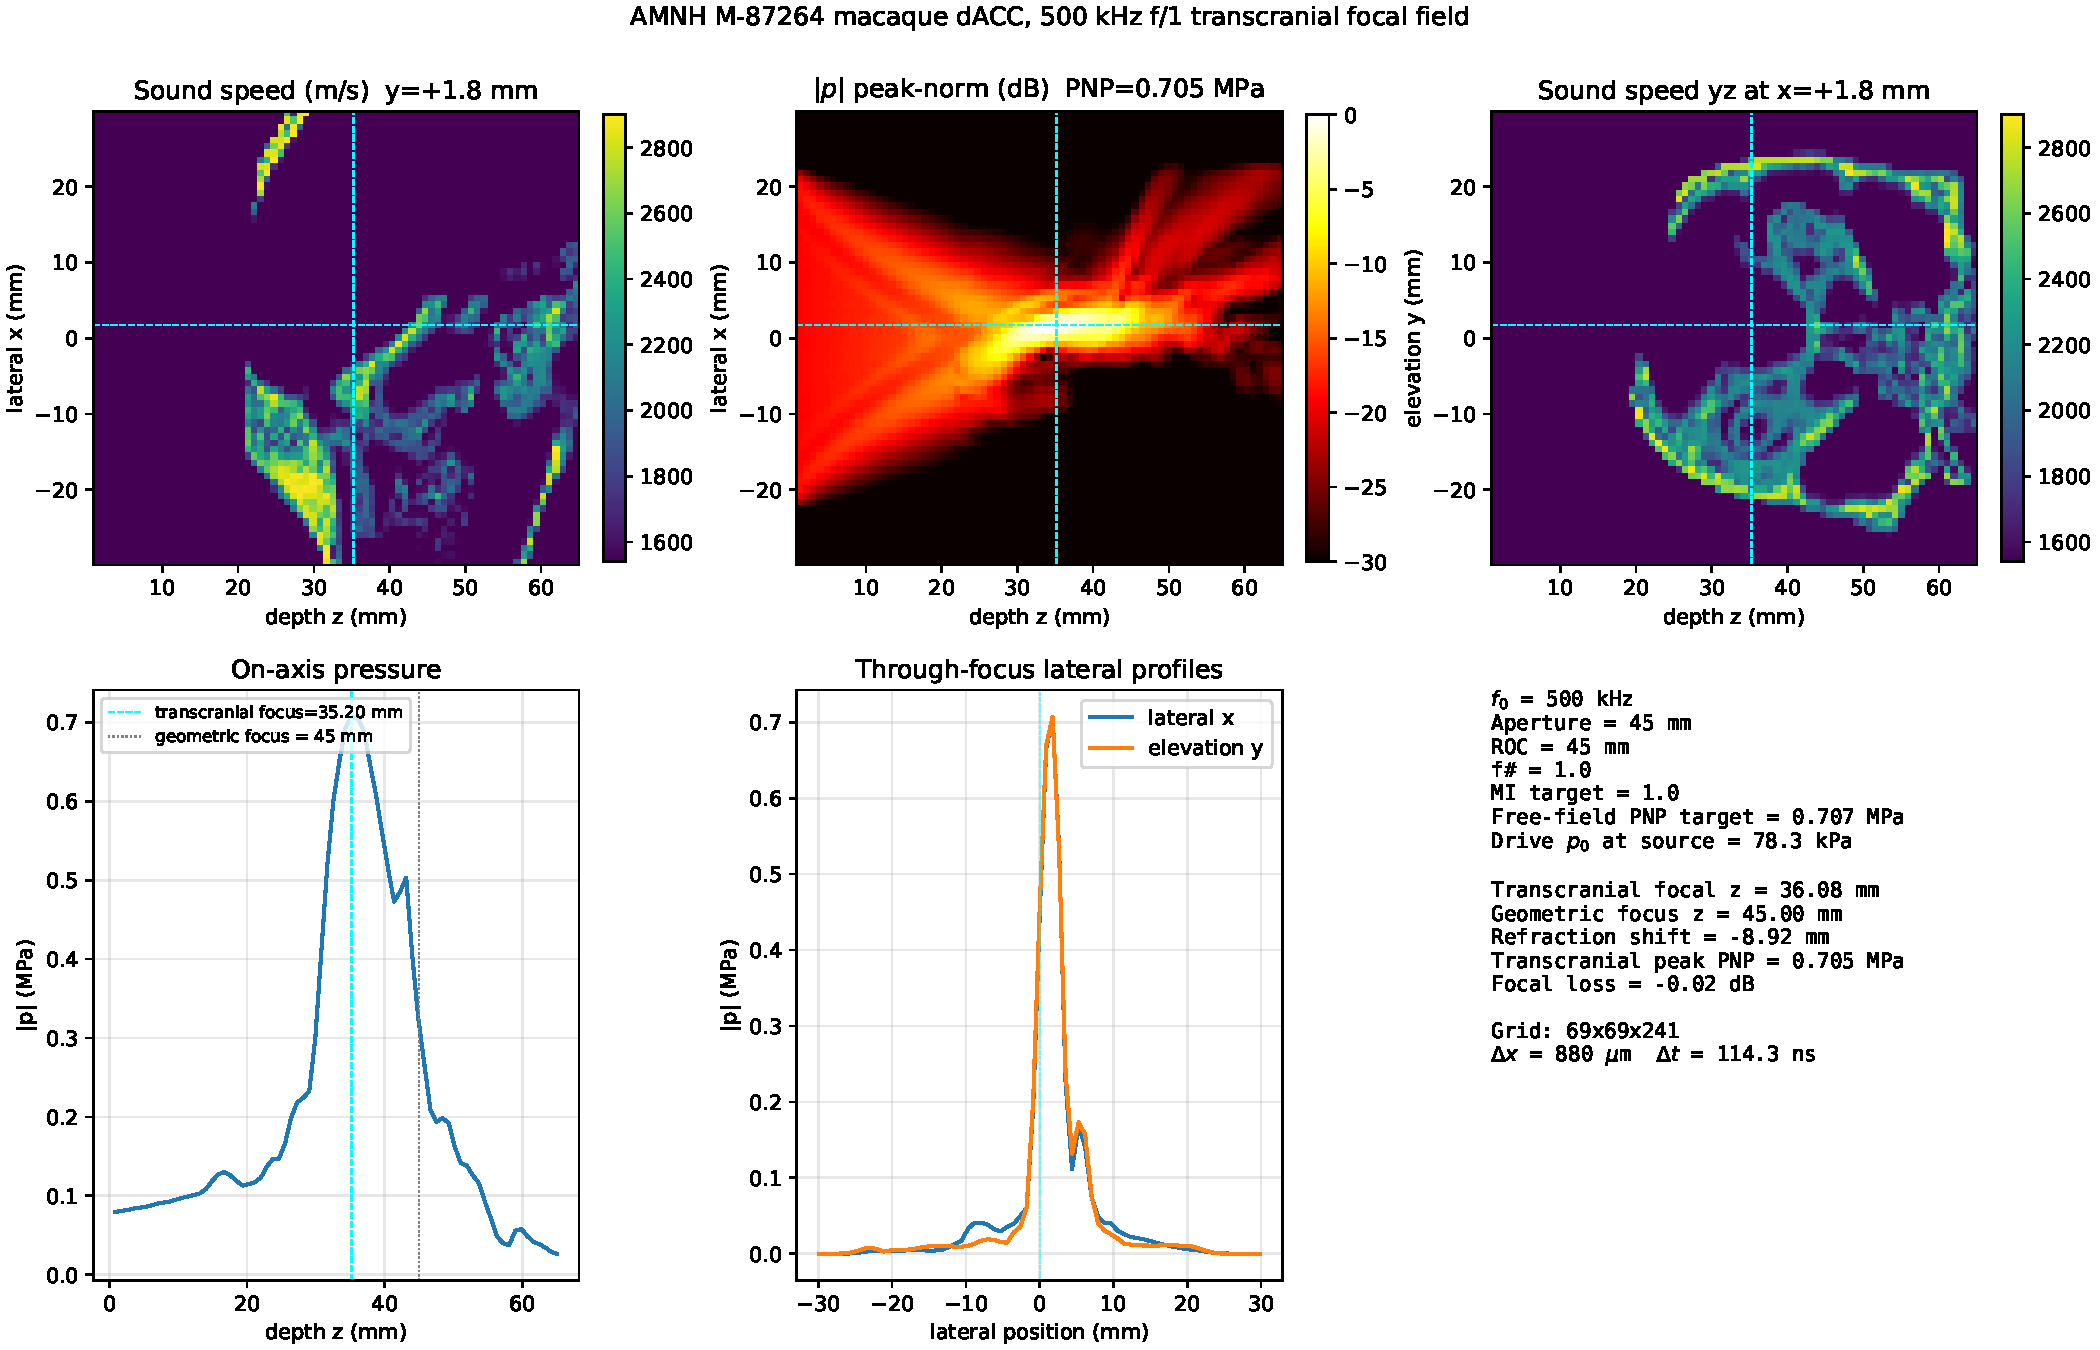
\includegraphics[width=\textwidth]{focal_field.pdf}
\caption{Macaque dACC focal-prediction summary. \textbf{Top row}:
         sound-speed cross-section ($xz$ at $y$\,=\,focal-peak),
         peak-normalised $|p|$ in dB on the same slice, and a $yz$
         sound-speed slice. \textbf{Bottom left}: on-axis pressure
         profile, with the geometric focus (45\,mm, grey dotted) and
         transcranial focus (37.0\,mm, cyan dashed) marked.
         \textbf{Bottom centre}: through-focus lateral profiles in $x$
         and $y$. \textbf{Bottom right}: simulation parameter summary.}
\label{fig:focal-field}
\end{figure}

\paragraph{What this does not measure.}
The result is a single transcranial run with no homogeneous reference,
so the only reportable focal-loss number is relative to the
free-field MI target by construction (which the drive calibration
forces to $0$\,dB). A complete validation would (i) add a homogeneous
free-field run at the same $p_0$ to extract the actual transcranial
insertion loss, (ii) sweep the bowl placement (sagittal tilt, lateral
search radius) for sensitivity to operator placement choice, and
(iii) anchor the absolute attenuation calibration with a transcranial
transmission measurement at 500\,kHz on the AMNH skull or a
representative second specimen. These are deferred to follow-up work.

% =============================================================================

\begin{thebibliography}{99}
\bibitem{copes-sci-data-2016} L.\,E.~Copes, L.\,A.~B.~Lucas,
  J.\,O.~Thostenson, H.\,E.~Hoekstra, and D.\,M.~Boyer,
  ``A collection of non-human primate computed tomography scans housed
  in MorphoSource, a repository for 3D data,''
  \emph{Sci.\ Data} {\bf 3}, 160001 (2016), doi:10.1038/sdata.2016.1.
\bibitem{nmt-v2} B.~Jung, P.\,A.~Taylor, J.~Seidlitz \emph{et al.},
  ``A comprehensive macaque fMRI pipeline and hierarchical atlas,''
  \emph{NeuroImage} {\bf 235}, 117997 (2021).
\bibitem{d99} K.\,S.~Saleem and N.~Logothetis, \emph{A Combined MRI and
  Histology Atlas of the Rhesus Monkey Brain in Stereotaxic
  Coordinates}, 2nd ed., Academic Press (2012); D99~v2 NMT-aligned
  release in \cite{nmt-v2}.
\bibitem{charm} B.~Jung, P.\,A.~Taylor, J.~Seidlitz \emph{et al.},
  ``Cortical Hierarchy Atlas of the Rhesus Macaque (CHARM),''
  \emph{NeuroImage} {\bf 224}, 117625 (2020).
\bibitem{sarm} D.~M.~Hartig, B.~Jung \emph{et al.},
  ``The Subcortical Atlas of the Rhesus Macaque (SARM),''
  \emph{NeuroImage} {\bf 235}, 117996 (2021).
\bibitem{folloni} D.~Folloni, L.~Verhagen, R.\,B.~Mars \emph{et al.},
  ``Manipulation of subcortical and deep cortical activity in the
  primate brain using transcranial focused ultrasound stimulation,''
  \emph{Neuron} {\bf 101}(6), 1109--1116.e5 (2019).
\bibitem{khalighinejad} N.~Khalighinejad, M.~Bongioanni, L.~Verhagen
  \emph{et al.},
  ``A basal forebrain-cingulate circuit in macaques decides it is time
  to act,'' \emph{Sci.\ Adv.} {\bf 6} (2020).
\bibitem{verhagen} L.~Verhagen, C.~Gallea, D.~Folloni \emph{et al.},
  ``Offline impact of transcranial focused ultrasound on cortical
  activation in primates,'' \emph{eLife} {\bf 8}, e40541 (2019).
\bibitem{badran} B.\,W.~Badran \emph{et al.},
  ``Low-intensity transcranial focused ultrasound to the dorsal
  anterior cingulate attenuates acute pain perception,''
  \emph{J.\ Neurosci.} {\bf 44}(8), e1011232023 (2024).
\bibitem{rhesus-volume} M.~Rilling, R.~Insel \emph{et al.}; published
  ranges: 70-110\,mL for adult \emph{Macaca mulatta}; mean ${\sim}$85\,mL
  with male/female sexual dimorphism (males trend high).
\bibitem{maga-validation} G.~F.~Pinton,
  ``Migrating the 15\,MHz transcranial mouse pipeline from DigiMouse to
  the Maga (UW) 4K microCT,'' validation report
  \texttt{mouse\_therapy/validation\_report\_maga/manuscript.tex},
  University of North Carolina at Chapel Hill (2026).
\end{thebibliography}

\end{document}
